\documentclass[preprint,12pt,aps,pra,showkeys,amsmath,amssymb,superscriptaddress,floatfix]{revtex4-2}
\usepackage[T1]{fontenc}
\usepackage[utf8]{inputenc}
\usepackage{amsmath,amssymb,amsthm,mathtools,mathrsfs}
\usepackage{microtype,booktabs,enumitem}
\usepackage{xcolor,tikz,etoolbox}
\usepackage[skins,breakable]{tcolorbox}
\usepackage{needspace}
% Keep diagram geometry independent of REVTeX preprint body spacing.
\AtBeginEnvironment{tikzpicture}{\linespread{1}\selectfont}
\usetikzlibrary{arrows.meta,positioning,calc,fit,decorations.pathreplacing}
\usepackage{graphicx}
\usepackage{hyperref}

\definecolor{MMBlue}{RGB}{0,82,155}
\definecolor{MMOrange}{RGB}{200,80,0}
\tikzset{
 mmnode/.style={draw=MMBlue,rounded corners=2pt,fill=MMBlue!4,align=left,execute at begin node={\raggedright},text width=5cm,font=\fontsize{10}{12}\selectfont,inner sep=6pt},
 mmimport/.style={mmnode,draw=black!65,fill=black!4},
 mmcandidate/.style={mmnode,draw=MMOrange,dashed,fill=MMOrange!5},
 mmrejected/.style={mmnode,draw=black,densely dotted,fill=black!8},
 mmproof/.style={->,thick,MMBlue},
 mmflow/.style={->,semithick,black!70},
 mmrepair/.style={->,dashed,thick,MMOrange},
 mmcandidatearrow/.style={->,dashed,semithick,MMOrange},
 mmnote/.style={font=\scriptsize,fill=white,inner sep=2pt,align=center}}

\usepackage[section]{placeins}
\setlength{\emergencystretch}{3em}
\setlist{itemsep=3pt,topsep=4pt}
\newtheorem{theorem}{Theorem}[section]
\newtheorem{proposition}[theorem]{Proposition}
\newtheorem{lemma}[theorem]{Lemma}
\newtheorem{corollary}[theorem]{Corollary}
\theoremstyle{definition}
\newtheorem{definition}[theorem]{Definition}
\newtheorem{example}[theorem]{Example}
\theoremstyle{remark}
\newtheorem{remark}[theorem]{Remark}
% Avoid isolated statement headings and single-line paragraph fragments.
\BeforeBeginEnvironment{theorem}{\Needspace{6\baselineskip}}
\BeforeBeginEnvironment{definition}{\Needspace{5\baselineskip}}
\BeforeBeginEnvironment{proposition}{\Needspace{5\baselineskip}}
\BeforeBeginEnvironment{lemma}{\Needspace{5\baselineskip}}
\BeforeBeginEnvironment{corollary}{\Needspace{5\baselineskip}}
\clubpenalty=5000
\widowpenalty=5000
\newcommand{\R}{\mathbb R}\newcommand{\Z}{\mathbb Z}\newcommand{\N}{\mathbb N}
\newcommand{\Pa}{\operatorname{Pa}}\newcommand{\Desc}{\operatorname{Desc}}
\newcommand{\cl}{\operatorname{cl}}\newcommand{\cost}{\operatorname{cost}}
\newcommand{\status}{\operatorname{status}}
% Faculty cards: a visual rail groups the five faculties within one agent.
% The rail has no arrowhead and does not represent a proof dependency.
\newcommand{\mmfacultybadge}[1]{%
 \node[circle,draw=MMBlue,line width=1pt,fill=white,
 minimum size=7mm,inner sep=0pt,font=\sffamily\small\bfseries,text=MMBlue]
 at ([xshift=15pt,yshift=-15pt]frame.north west) {#1};}
\newcommand{\mmfacultyrail}{%
 \draw[MMBlue!80,line width=1pt]
 ([xshift=15pt,yshift=2pt]frame.north west)--
 ([xshift=15pt,yshift=-2pt]frame.south west);}
\newtcolorbox{mmfacultybox}[2]{enhanced,breakable,
 colback=MMBlue!4,colframe=MMBlue!4,boxrule=0pt,arc=3pt,
 left=39pt,right=9pt,top=4pt,bottom=4pt,
 before skip=2pt,after skip=2pt,
 fontupper=\small\linespread{1.1}\selectfont,
 overlay unbroken={\mmfacultyrail\mmfacultybadge{#1}},
 overlay first={\mmfacultyrail\mmfacultybadge{#1}},
 overlay middle={\mmfacultyrail},overlay last={\mmfacultyrail}}
\newcommand{\mmfaculty}[3]{%
 \begin{mmfacultybox}{#1}{#2}
 {\sffamily\bfseries\color{MMBlue}#2}\par\smallskip #3
 \end{mmfacultybox}}
\newcommand{\agent}[9]{%
 \Needspace{8\baselineskip}
 \subsubsection{#1}
 \noindent\textbf{Object.} #2\par
 \noindent\textbf{Role.} #3\par\smallskip
 \mmfaculty{E}{Ego}{#4}
 \mmfaculty{M}{Memory}{#5}
 \mmfaculty{I}{Intellect}{#6}
 \mmfaculty{S}{Sense}{#7}
 \mmfaculty{A}{Action}{#8}
 \smallskip\noindent #9\par}

\usepackage{longtable,array,calc}
\providecommand{\tightlist}{\setlength{\itemsep}{2pt}\setlength{\parskip}{0pt}}
\makeatletter
\def\frontmatter@abstract@produce{\par\addvspace{\frontmatter@preabstractspace}%
\begingroup\prep@absbox\unvbox\absbox\post@absbox\endgroup
\addvspace{\frontmatter@postabstractspace}}
\makeatother
\newcommand{\field}[2]{\par\smallskip\noindent\textbf{#1.} #2\par}
\setlength{\emergencystretch}{5em}
\AtBeginEnvironment{verbatim}{\small\linespread{1.0}\selectfont}


\hypersetup{colorlinks=true,linkcolor=MMBlue,urlcolor=MMBlue,pdfauthor={Dibakar Sigdel}}

\begin{document}

\title{Global Gauss--Bonnet Theorem for Surfaces\\[4pt]\large An End-to-End Meta-Math Walkthrough}

\author{Dibakar Sigdel}

\affiliation{Mindverse Computing LLC, Lynnwood, WA 98087, USA}

\date{October 2026}

\begin{abstract}

A complete authored walkthrough of global gauss--bonnet theorem for
surfaces, with explicit mathematical contracts, local verification
gates, and reusable exports. The report presents the target theorem,
declared imports, a dependency graph, five-faculty node contracts, a
continuous proof, a worked example, and a hypothesis-repair audit. It is
an authored mathematical exposition, not a deployed-agent transcript or
a formal proof-assistant certificate.

\end{abstract}\maketitle\linespread{1.12}\selectfont

\noindent\textbf{DG-04 / Differential Geometry / Report v1}

\section{Target and import contract}

\begin{theorem}

For a closed oriented smooth Riemannian surface \(M\), prove
\(\int_M K\,dA=2\pi\chi(M)\). Here closed means compact without
boundary.

\end{theorem}

\subsection{Foundations and permitted imports}

Import local Gauss--Bonnet for an oriented disk-like region with
piecewise smooth positively oriented boundary: \(\int K\)
\(dA+\int boundary\) \(k_g\) \(ds+\sum\) exterior turning
\(angles=2\pi\). Also import a finite smooth triangulation of the closed
oriented surface with regular edges and tangent sectors \(filling2\pi\)
around every vertex. Curvature is intrinsic by DG-03. These local
geometric and triangulation modules are substantial imports; the global
formula is proved by assembly.

For an abstract Riemannian surface, \(K\) is defined intrinsically from
its Levi-Civita curvature tensor. DG-03 explains the agreement with
extrinsic Gaussian curvature on embedded surfaces; its extrinsic
statement is context, not a necessary premise of this assembly proof.

\clearpage\section{Node interaction workflow}

\begin{center}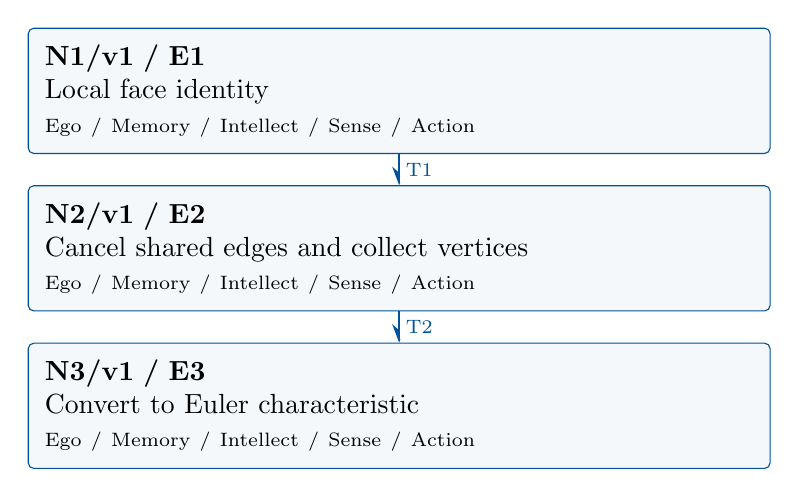
\begin{tikzpicture}[>=Stealth,x=1cm,y=1cm]

\node[mmnode,text width=9cm,minimum height=1.25cm] (N1) at (0,0.0) {\textbf{N1/v1 / E1}\\Local face identity\\{\scriptsize Ego / Memory / Intellect / Sense / Action}};

\node[mmnode,text width=9cm,minimum height=1.25cm] (N2) at (0,-2.0) {\textbf{N2/v1 / E2}\\Cancel shared edges and collect vertices\\{\scriptsize Ego / Memory / Intellect / Sense / Action}};

\node[mmnode,text width=9cm,minimum height=1.25cm] (N3) at (0,-4.0) {\textbf{N3/v1 / E3}\\Convert to Euler characteristic\\{\scriptsize Ego / Memory / Intellect / Sense / Action}};

\draw[mmproof] (N1.south) -- node[mmnote,right] {T1} (N2.north);

\draw[mmproof] (N2.south) -- node[mmnote,right] {T2} (N3.north);

\end{tikzpicture}\end{center}

Each box is one mathematical agent containing all five faculties. Blue
arrows carry the versioned exports listed below. The layout gives a
reading order; only drawn arrows assert dependencies. Diagnostic repair
is separate from the proof DAG.

\subsection{Versioned evidence-transfer ledger}

\begingroup\small\linespread{1.05}\selectfont

\Needspace{5\baselineskip}\field{T1: N1/E1/v1 to N2}{A local curvature identity for each face.}

\field{Receiving activity}{N2: Cancel shared edges and collect vertices}

\field{Compatibility}{Use the same mathematical objects and hypotheses as the source export.
Receiving contract: All local face identities; closed oriented surface;
prior exports E1/v1}

\Needspace{5\baselineskip}\field{T2: N2/E2/v1 to N3}{The global integral equals \(2\pi V-\pi F\).}

\field{Receiving activity}{N3: Convert to Euler characteristic}

\field{Compatibility}{Use the same mathematical objects and hypotheses as the source export.
Receiving contract: Triangulation counts; prior exports E2/v1}

\endgroup

\clearpage\section{Agent roles and five-faculty activities}\begingroup\small\linespread{1.05}\selectfont\setlist{itemsep=1pt,topsep=2pt}

\subsection{N1/v1: Local face identity}

\field{Object and role}{Express turning angles through interior face angles.}

\field{Inputs}{A compatible finite triangulation; foundational imports stated in §1}

\mmfaculty{E}{Ego}{Own E1/v1: A local curvature identity for each face.}

\mmfaculty{M}{Memory}{Retain A compatible finite triangulation; foundational imports stated in
§1; keep their assumptions and versions attached.}

\mmfaculty{I}{Intellect}{Express turning angles through interior face angles.}

\mmfaculty{S}{Sense}{Do not silently assume every triangulation edge is geodesic.}

\mmfaculty{A}{Action}{Carry out the numbered deductions and publish E1/v1 together with its
hypotheses and proof location.}

\smallskip\noindent\textbf{Numbered mathematical activities}

\begin{enumerate}[label=N1.\arabic*,leftmargin=3.4em]

\item For each triangular faceF with interior corner angles \(\theta _{Fv}\),
the local theorem reads \(\int _F\) \(KdA+\int _\partial F\)
\(k_gds+\sum _{v\in F}(\pi -\theta _{Fv})=2\pi\).

\item The boundary need not be geodesic: retain its geodesic-curvature term.

\item Each face is disk-like and all boundary orientations are the induced
positive ones.

\end{enumerate}

\field{Export E1/v1}{A local curvature identity for each face.}

\field{Acceptance gate}{Do not silently assume every triangulation edge is geodesic. Publish
only after checking every displayed deduction.}

\field{Targeted repair}{If the check fails, revise N1: Do not silently assume every
triangulation edge is geodesic. Recheck dependent nodes N2, N3.}

\clearpage

\subsection{N2/v1: Cancel shared edges and collect vertices}

\field{Object and role}{Pair each edge with its opposite boundary orientation.}

\field{Inputs}{All local face identities; closed oriented surface; prior exports E1/v1}

\mmfaculty{E}{Ego}{Own E2/v1: The global integral equals \(2\pi V-\pi F\).}

\mmfaculty{M}{Memory}{Retain All local face identities; closed oriented surface; prior exports
E1/v1; keep their assumptions and versions attached.}

\mmfaculty{I}{Intellect}{Pair each edge with its opposite boundary orientation.}

\mmfaculty{S}{Sense}{No boundary edge may remain unpaired; this uses that M is closed.}

\mmfaculty{A}{Action}{Carry out the numbered deductions and publish E2/v1 together with its
hypotheses and proof location.}

\smallskip\noindent\textbf{Numbered mathematical activities}

\begin{enumerate}[label=N2.\arabic*,leftmargin=3.4em]

\item Sum over the F faces.

\item Every edge belongs to two faces with opposite induced boundary
directions; its signed geodesic-curvature integrals cancel.

\item At each vertex the incident interior sectors sum to \(2\pi\).

\item There are 3F corner incidences, so the sum of all exterior angles is
\(3\pi F-2\pi V\).

\item Thus \(\int _M\) \(KdA+3\pi F-2\pi V=2\pi F\), yielding \(\int _M\)
\(KdA=2\pi V-\pi F\).

\end{enumerate}

\field{Export E2/v1}{The global integral equals \(2\pi V-\pi F\).}

\field{Acceptance gate}{No boundary edge may remain unpaired; this uses that M is closed.
Publish only after checking every displayed deduction.}

\field{Targeted repair}{If the check fails, revise N2: No boundary edge may remain unpaired;
this uses that M is closed. Recheck dependent nodes N3.}

\clearpage

\subsection{N3/v1: Convert to Euler characteristic}

\field{Object and role}{Count incidences before substituting \(\chi\).}

\field{Inputs}{Triangulation counts; prior exports E2/v1}

\mmfaculty{E}{Ego}{Own E3/v1: Global Gauss--Bonnet under the stated hypotheses.}

\mmfaculty{M}{Memory}{Retain Triangulation counts; prior exports E2/v1; keep their assumptions
and versions attached.}

\mmfaculty{I}{Intellect}{Count incidences before substituting \(\chi\).}

\mmfaculty{S}{Sense}{A surface with boundary needs additional boundary curvature and corner
terms.}

\mmfaculty{A}{Action}{Carry out the numbered deductions and publish E3/v1 together with its
hypotheses and proof location.}

\smallskip\noindent\textbf{Numbered mathematical activities}

\begin{enumerate}[label=N3.\arabic*,leftmargin=3.4em]

\item Because each triangle has 3 edges and each edge is shared by 2
\(triangles,3F=2E\).

\item Then \(2\pi (V-E+F)=2\pi V-\pi F\), the preceding integral.

\item Using \(\chi (M)=V-E+F\) gives \(\int K\) \(dA=2\pi \chi (M)\).

\item The formula is independent of the selected compatible triangulation;
\(\chi\) is its topological invariant.

\end{enumerate}

\field{Export E3/v1}{Global Gauss--Bonnet under the stated hypotheses.}

\field{Acceptance gate}{A surface with boundary needs additional boundary curvature and corner
terms. Publish only after checking every displayed deduction.}

\field{Targeted repair}{If the check fails, revise N3: A surface with boundary needs additional
boundary curvature and corner terms. Withhold this terminal result until
its gate passes.}

\endgroup\clearpage\section{Continuous mathematical proof}\label{sec:proof}

Read these steps in order as one proof; the diagram is optional.
Numbered activities identify the specific constructions and deductions
owned by each node.

\subsection{§4.N1 --- Local face identity}\label{n1-local-face-identity}

\begin{enumerate}
\def\labelenumi{\arabic{enumi}.}
\item
  For each triangular faceF with interior corner angles
  \(\theta _{Fv}\), the local theorem reads \(\int _F\)
  \(KdA+\int _\partial F\)
  \(k_gds+\sum _{v\in F}(\pi -\theta _{Fv})=2\pi\).
\item
  The boundary need not be geodesic: retain its geodesic-curvature term.
\item
  Each face is disk-like and all boundary orientations are the induced
  positive ones.
\end{enumerate}

\subsection{§4.N2 --- Cancel shared edges and collect
vertices}\label{n2-cancel-shared-edges-and-collect-vertices}

\begin{enumerate}
\def\labelenumi{\arabic{enumi}.}
\item
  Sum over the F faces.
\item
  Every edge belongs to two faces with opposite induced boundary
  directions; its signed geodesic-curvature integrals cancel.
\item
  At each vertex the incident interior sectors sum to \(2\pi\).
\item
  There are 3F corner incidences, so the sum of all exterior angles is
  \(3\pi F-2\pi V\).
\item
  Thus \(\int _M\) \(KdA+3\pi F-2\pi V=2\pi F\), yielding \(\int _M\)
  \(KdA=2\pi V-\pi F\).
\end{enumerate}

\subsection{§4.N3 --- Convert to Euler
characteristic}\label{n3-convert-to-euler-characteristic}

\begin{enumerate}
\def\labelenumi{\arabic{enumi}.}
\item
  Because each triangle has 3 edges and each edge is shared by 2
  \(triangles,3F=2E\).
\item
  Then \(2\pi (V-E+F)=2\pi V-\pi F\), the preceding integral.
\item
  Using \(\chi (M)=V-E+F\) gives \(\int K\) \(dA=2\pi \chi (M)\).
\item
  The formula is independent of the selected compatible triangulation;
  \(\chi\) is its topological invariant.
\end{enumerate}

\hfill$\square$

\section{Worked orchestration}

For the unit sphere, \(K=1\) and \(area4\pi\), so its integral is
\(4\pi =2\pi \cdot 2\). A tetrahedral combinatorial triangulation has
\(V=4,E=6,F=4\) and \(\chi =2\). A flat metric on the torus has \(K=0\)
and \(\chi =0\), giving a second consistency check.

\subsection{Boundary and hypothesis audit}

A flat unit disk has zero curvature integral but \(\chi =1\); its
boundary contributes \(\int k_gds=2\pi\). Sense rejects applying the
closed-surface formula to the disk and restores the boundary terms of
the local theorem.

\section{Illustrative failure and repair}

The following is an authored diagnostic scenario. Changed assumptions
define a new contract; they do not retroactively prove the original
statement.

\subsection{Failure and correction}
This is an authored teaching trace, not a recorded agent run.

\begin{enumerate}
\def\labelenumi{\arabic{enumi}.}
\tightlist
\item
  \textbf{Ego \(\to\) Memory:} register the §1 theorem, imports, and
  requested exports before beginning the proof.
\item
  \textbf{Intellect \(\to\) Action:} choose the bridges in §3 and carry
  out the numbered activities in §4; transmit only established E-exports
  along the §2 DAG.
\item
  \textbf{Sense \(\to\) responsible node:} test the specific
  boundary/failure in §5 and the node's individual audit. A failing
  candidate is withheld; downstream nodes may not use it.
\item
  \textbf{Memory + Intellect:} identify whether the error is an omitted
  condition, an invalid inference, or an attempted extension beyond the
  theorem. Restore the exact contract or explicitly state a different
  one.
\item
  \textbf{Action:} redo the affected mathematical activity using the
  repaired condition or inference. Recheck consuming nodes, rather than
  feeding their conclusions back as premises.
\item
  \textbf{Ego:} publish only the supported export with its assumptions
  and proof location. A hypothetical revised export is v2; the written
  proof here is the v1 exposition, not a claim that this repair was
  executed.
\end{enumerate}

\subsection{Hypothesis boundary}
A flat unit disk has zero curvature integral but \(\chi =1\); its
boundary contributes \(\int k_gds=2\pi\). Sense rejects applying the
closed-surface formula to the disk and restores the boundary terms of
the local theorem.

\subsection{Version and recheck}
Treat any changed assumption as a new contract. Recheck the revised
export and all of its descendants. A backward diagnostic never
establishes an earlier theorem. This is an authored teaching trace, not
an execution log.

\par\medskip\begingroup\small\linespread{1.0}\selectfont\noindent\textbf{Provenance.} This authored proof is complete relative to its declared imports. Reuse
each export with its assumptions, proof, and version. The original
Markdown remains available for comparison.
\par\endgroup

\par\smallskip\begingroup\small\linespread{1.0}\selectfont\noindent\textbf{Further reading.} \begin{itemize}
\tightlist
\item
  \href{https://ocw.mit.edu/courses/18-900-geometry-and-topology-in-the-plane-spring-2023/pages/chapter-ix-curved-geometries/}{MIT
  Geometry and Topology: curved geometries and Gauss--Bonnet}.
\end{itemize}\par\endgroup

\end{document}
